% begin module function-def
\begin{frame}

\ \only<handout:0| 1>{%
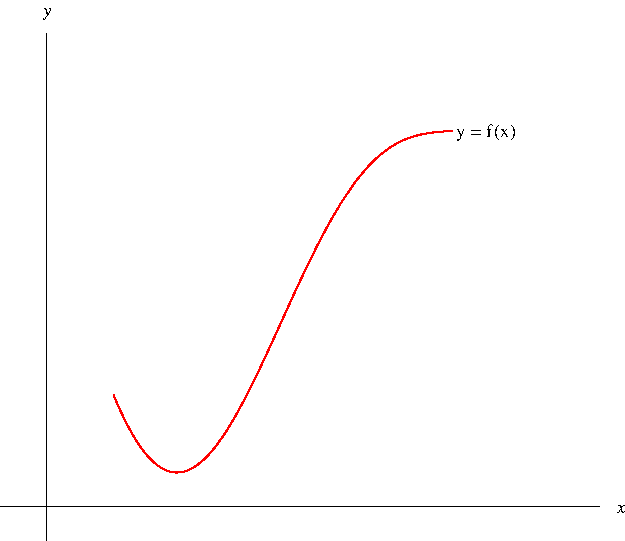
\includegraphics[height=5cm]{precalculus/pictures/01-01-function.pdf}
}%
\only<handout:1| 2>{%
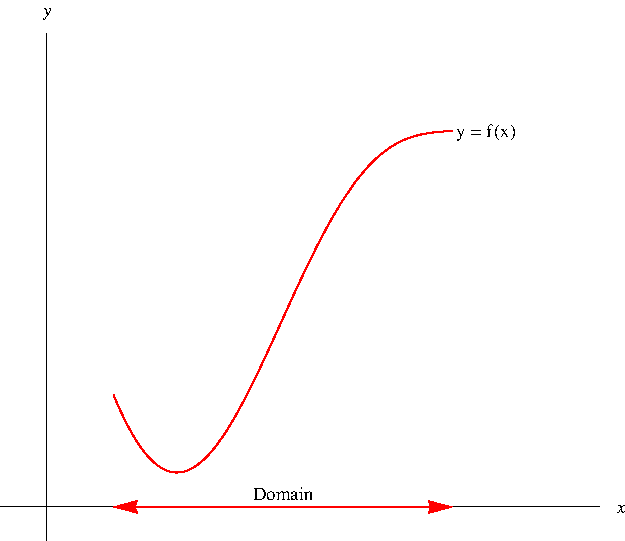
\includegraphics[height=5cm]{precalculus/pictures/01-01-domain.pdf}
}%
\only<handout:2| 3>{%
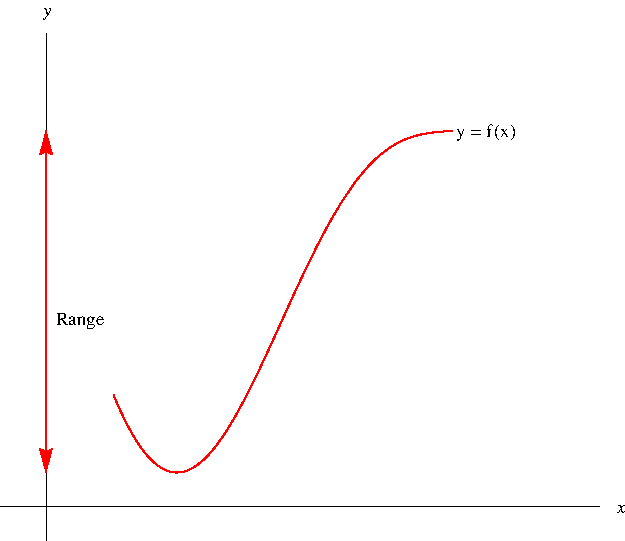
\includegraphics[height=5cm]{precalculus/pictures/01-01-range.pdf}
}%
\only<handout:3-| 4->{%
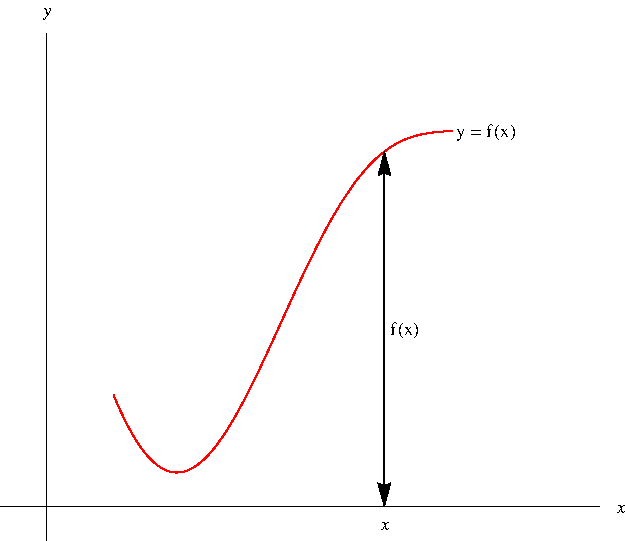
\includegraphics[height=5cm]{precalculus/pictures/01-01-fofx.pdf}
}%

\begin{definition}[Function]
A function $f$ is a rule that assigns to each element $x$ in a set $D$ exactly one element, called $f(x)$, in a set $E$.
\end{definition}

\uncover<2>{
\only<handout:1| -2>{
\begin{definition}[Domain]
The set $D$ is called the domain. 
\end{definition}
}
}

\only<handout:2| 3>{
\begin{definition}[Range]
The set $E$ is called the range. 
\end{definition}
}

\only<handout:3| 4->{
\begin{definition}[Value of $f$ at $x$]
The number $f(x)$ is called the value of $f$ at $x$, and is read ``$f$ of $x$.''
\end{definition}
}
\end{frame}
% end module function-def
